\listfiles
\documentclass[12pt,a4paper]{article}

%% Bibliography style:
\usepackage[pdftex]{graphicx}
\usepackage{amsmath}
\usepackage{array}

\usepackage[a4paper,margin=1in]{geometry}

%% Natbib is a popular style for formatting references.
%\usepackage[numbers]{natbib}
%% bibpunct sets the punctuation used for formatting citations.
%\bibpunct{(}{)}{;}{a}{,}{,}

\setlength{\parskip}{1.5ex plus 0.5ex minus 0.2ex}
\linespread{0}

\title{State Merging for Automatic Test Generation}
\date{}

\author{
Kuan Xiang Wen$^{1}$, Li Xuan Ji$^{1}$, Tan Jiaqi$^{2}$\\
\vspace{1 mm} \\
\small{$^{1}$NUS High School of Math and Science}\\
\small{$^{2}$INFO Division, DSO National Laboratories, Singapore}
}

\newcommand{\klee}{\textsc{klee}}
\newcommand{\leek}{\textsc{leek}}


\begin{document}
\maketitle
\begin{abstract}
Automatic test generation is the problem of generating test cases in a given program for the purposes of vulnerability detection and program verification. One method of achieving this is Symbolic Execution, which executes the program with \emph{symbolic} variables to quickly test every possible execution path that the program may take. Often symbolic execution creates many execution paths that are similar; our project focuses on determining when these paths can be merged to cut down on repetitive operations. In addition, we have developed a pseudomerging algorithm to avoid situations where the merging algorithm performes worse. We prove our algorithm's correctness and optimality and demonstrate its practical usefulness by generating test cases for real world programs. We observe speed up from exponential to linear time for certain programs.
\end{abstract}

\section{Introduction}
Testing is very important. We spend a lot of money on it. Unfortunately, the only widely used methods to generate test cases are a) manually writing them and b) generating them randomly through fuzz testing. Manually writing them is expensive and boring, while generating them randomly has been shown to result in low program coverage. 

Automatic test generation aims to solve this problem by using a computer to generate the test cases for a given program. The main approach to solving it is symbolic execution: we mark the input to the program as symbolic, ie, it can be anything, and we execute the program code on this symbolic input. When there is a conditional branch in the program, the system splits execution state into two, one where the branch guard is constrained to be true and one where it is false. Because only a small portion of execution paths are actually possible, a SMT solver is used to discard un-executable paths. 

In our work, we extend a state-of-the-art symbolic execution engine, \klee, developed at Stanford Univeristy. \klee is written in C++ and runs on LLVM bitcode. It is good.

\paragraph{Outline}

The remainder of this article is organized as follows. \S\ref{overview} presents a case study demonstrating the key features of our algorithm. \S\ref{algorithm} describes our algorithm while \S\ref{implementation} describes our implementation. Our results are described in \S\ref{evaluation}. Finally, \S\ref{conclusions} gives the conclusions.

\section{Overview}\label{overview}
Here is an example of a test program we used, Berkeley Packet Filter (or bpf for short), to illustrate our merging algorithm.

\begin{verbatim}
1. int bpf_validate(struct bpf_insn *f, int len)
2. {
3.      int i;
4.      int from;
5.      struct bpf_insn *p;
6.      if (len < 1 || len > BPF_MAXINSNS)
7.         return 0;
8.      for (i = 0; i < len; ++i) {
9.         p = &f[i];
10.        switch (BPF_CLASS(p->code)) {
11.        case BPF_LD:
12.        case BPF_LDX:
13.            switch (BPF_MODE(p->code)) {
14.            case BPF_IMM:
15.            ...
16.            }
17.        break;
18.        case BPF_ST:
19.        ...
20.        }
21.     }
22.     return BPF_CLASS(f[len - 1].code) == BPF_RET;
23. }
24. #define N 10 
25. int main(int argc, char *argv[]){  
26.
27.  struct bpf_insn ins_buffer[N];
28.
29.  klee_make_symbolic(ins_buffer, N * sizeof(ins_buffer[0]), "lol");
30.  return bpf_validate(ins_buffer, N);
31.}
\end{verbatim}

\begin{enumerate}
\item The variable ins\_buffer is marked as symbolic in ln29. 
\item In line 8, the for-loop creates a fork, one where the guard is true and one where it is false. Each time the for-loop is run, there will be a new fork, creating new execution states. 
\item At line 10, the switch statement forks execution $N-1$ times, where $N$ is the number of case statements
\item At line 13, the nested switch statementA Region is a connected subgraph of a control flow graph that has exactly two connections to the remaining graph. will create more execution states. 
\item When the first execution state reaches line 20, it will not continue executing.
\item When all execution states reach line 20, our algorithm will merge all of them, since their constraints do not differ much.
\end{enumerate}

This means that if a single execution state enters the loop body, all the execution states created by branching from it will merge back with it at the end of the switch statement, so no net additional execution states are created. In contrast, \klee creates $N-1$ new execution states and does not merge them back. This means \klee will create $N^\text{len} - 1$ execution states and will have exponential complexity, while our algorithm has linear complexity.

The main challenge our algorithm solves is determining when an execution state must pause. If an execution state is executed past the merge point (at line 20) then a chance to merge is missed.

\section{Algorithm}\label{algorithm}
In order to minimize the number of execution paths, we aim to merge the similar execution paths. We have primarily 2 major operations: simplifying and merging. The simplifying function takes the multiple constraints from the different execution paths and, using some set theory, simplifies them into something smaller that is easier for the merge function to handle. The merge function itself uses a mix of several libraries with its own algorithm to determine when and where is suitable to merge such that the process will be without loss of completeness.

\begin{figure}[h!]
  \centering
    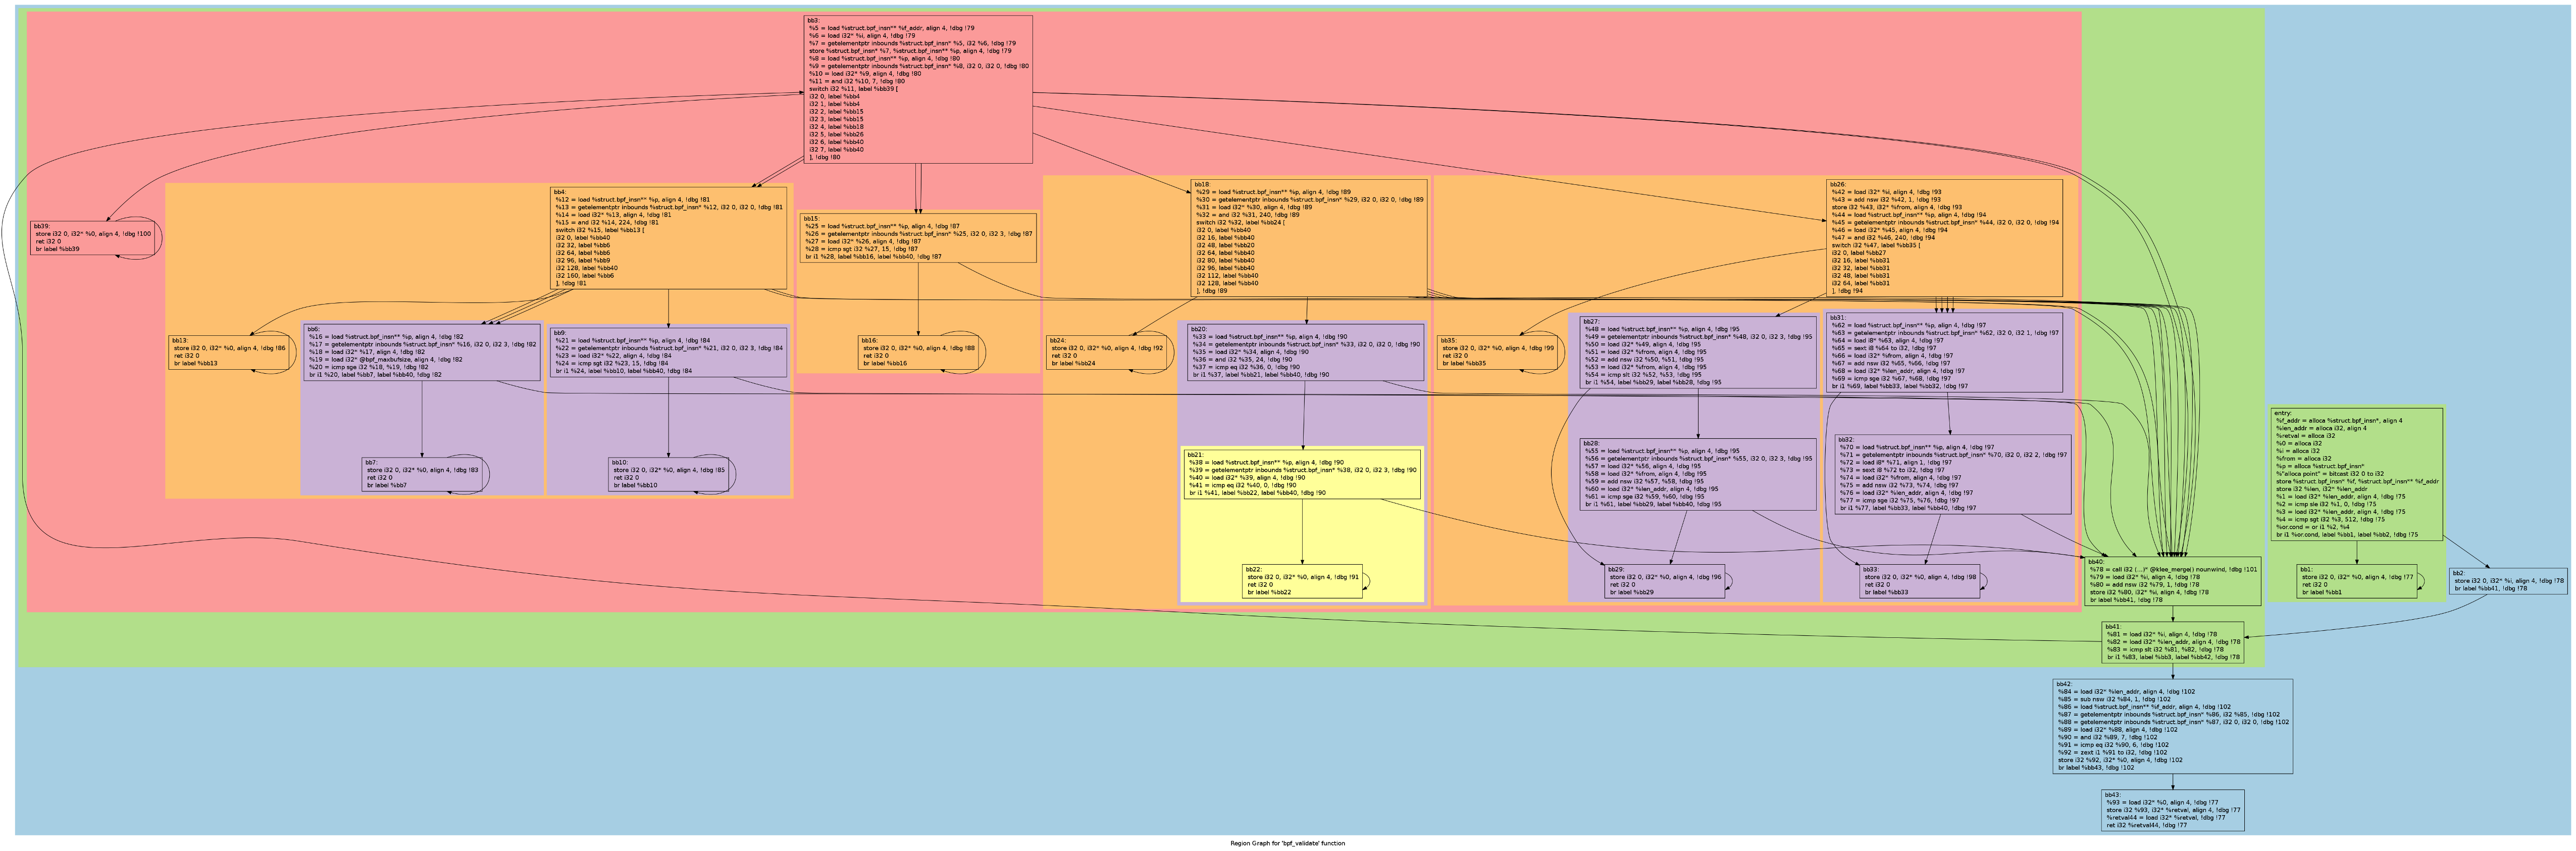
\includegraphics[width=\textwidth]{reg.png}
  \caption{Region information for bpf\_validate overlaid on the CFG. Each box is a \emph{basic block}; those in the same region are grouped by colour.}
\end{figure}

\subsection{Merge}
Internally, LLVM bitcode consists of \textbf{Basic Blocks}, which are blocks of straigt-line code terminated by a control flow instruction. The control flow graph has basic blocks as nodes and directed edges representing control flow. We then group the basic blocks into \emph{Regions}. A Region is a connected subgraph of a control flow graph that has exactly two connections to the remaining graph; regions may be nested. 

In our algorithm, we track the regions an execution state is in. Whenever an execution path leaves a region $R$, it pauses and waits for other states in $R$ to leave $R$. Then, it tries to merge with other states paused at the same point before continuing.

%A problem that arises is that \emph{return} are similar to \emph{goto} statements. A \emph{return} statement forces an execution state to point straight toward the end of the program. Hence, what could have been a region, has another 'exit' and does not fufil the 'one-entry-one-exit' rule. As a result, no merging will be done. This problem is common as many real-world programs uses switch-case statements with \emph{return} statements inside. To curb this problem, we harmlessly tweak the \emph{return} statements, such that each return statement has a fake infinite loop such that they will not point to the end of the program. This infinite loop is put after the return statement, hence will never be executed, but the tree will change such that there will not be an additional exit, thus and the region will be able to be created.

\paragraph{When to merge?}
We discovered experimentally that if we always merge execution states whenever possible, \klee takes a much longer time to solve the resulting constraints, outweighing the speedups offered by merging.

\subsection{Simplify}
The first part of our simplifier uses a principle that we developed ourselves:
Consider an expression $E = A\cap(B\cup A)$. We consider cases: if $A$ were false, then E will be false regardless of the value of $(B\cup A)$. If $A$ were true, we can replaces occurences of $A$ in the RHS with true. Thus we can always replace occurences of $A$ in the RHS with true. The tree will then simplify to $A\cap(B\cup \text{True}) = A$. By duality, in $A\cup(B\cup A)$ we can replace occurances of $A$ in $(B\cup A)$ by false.

In the second part of the simplifier algorithm, we use simple theorems for simplification (eg. $A\cup \text{True} = \text{True}$) to complete the simplification. The simplifier algorithm will be repeatedly run until the expression does not change.

\section{Implementation}\label{implementation}
In this section we describe the results.

\section{Evaluation}\label{evaluation}
We evaluated \textsc{leek} by selecting 12 benchmarks that were used in the literature before \cite{boom} \cite{boom}.

\begin{center}
\setlength{\extrarowheight}{2ex}
\begin{tabular}{|m{5.5cm} *{4}{| m{1.7cm} }|}
\hline
Name & LOC & Size & \multicolumn{2}{p{3.4cm}|}{Time Taken}\\ \cline{4-5}
 & & & \multicolumn{1}{p{1.7cm}|}{\klee} & \multicolumn{1}{p{1.7cm}|}{\leek}\\ \hline
netbsd/glob2 & 42 & 40 & 1.842 & 0.586\\ \hline
apache/get\_tag & 42 & 10 & 66.164 & 62.467\\ \hline
%apache/escape\_absolute\_uri & 42 & 10 & 66.164 & 62.467\\ \hline
bpf/bpf\_validate & 42 & 100 & 254.625 & 6.258\\ \hline
mult\cite{boom} & 42 & 1 & 7.264 & 0.111\\ \hline
edbrowse/ftpls & 42 & 32 & 91.369 & 13.937\\ \hline

\end{tabular}
\end{center}

Furthermore, we performed two other small experiments. Firstly, we measuerd time taken to analyze a program as a function on the number of bytes made symbolic for both \klee \ and \leek. 

\section{Conclusions}\label{conclusions}
We see that in programs with nested loops and switch statements in loops, the merge algorithm helps \klee to take much less time to finish debugging the program.

Implications: Rather than just an algorithm for \klee, our algorithm itself is a good method for programs that 

We also should consider to extend the merge algorithm to cater to the messy goto() statements which, as mentioned in \S\ref{algorithm}, disallows regions from being created. \cite{lamport94}

This too \cite{boom}. \klee is good.

\section{Appendix}
\klee: Unassisted and Automatic Generation of High-Coverage Tests for Complex Systems Programs

%\bibliographystyle{plain}
%\bibliography{ref}
EXE: Automatically Generating Inputs of Death - www.stanford.edu/~engler/exe-ccs-06.pdf

\begin{thebibliography}{9}

\bibitem{lamport94}
         Leslie Lamport,
          \emph{\LaTeX: A Document Preparation System}.
	  Addison Wesley, Massachusetts,
	  2nd Edition,
	  1994.

\bibitem{boom}
         HIM
         \emph{\textsc{klee}: Unassisted and Automatic Generation of High-Coverage Tests for Complex Systems Programs}
         Stanford
\end{thebibliography}



\end{document}
